%%%%%%%%%%%%%%%%%%%%%%%%%%%%%%%%%%%%%%%%%%%%%%%%%%%%%%%%%%%%%%%%%%%%%%%
% Sample template for MIT Junior Lab Student Written Summaries
% Available from http://web.mit.edu/8.13/samplepaper/sample-paper.tex
%
% Last Updated June 20, 2004
%
% Adapted from the American Physical Societies REVTeK-4 Pages
% at http://publish.aps.org
%
% ADVICE TO STUDENTS: Each time you write a paper, start with this
%    template and save under a new filename.  If convenient, don't
%    erase unneeded lines, just comment them out.  Often, they
%    will be useful containers for information.
%%%%%%%%%%%%%%%%%%%%%%%%%%%%%%%%%%%%%%%%%%%%%%%%%%%%%%%%%%%%%%%%%%%%%%%


%%%%%%%%%%%%%%%%%%%%%%%%%%%%%%%%%%%%%%%%%%%%%%%%%%%%%%%%%%%%%%%%%%%%%%%
% PREAMBLE
% The preamble of a LaTeX document is the set of commands that precede
% the \begin{document} line.  It contains a \documentclass line
% to load the REVTeK-4 macro definitions and various \usepackage
% lines to load other macro packages.
%
% ADVICE TO STUDENTS: This preamble contains a suggested set of
%     class options to generate a ``Junior Lab'' look and feel that
%     facilitate quick review and feedback from one's peers, TA's
%     and section instructors.  Don't make substantial changes without
%     first consulting your section instructor.
%%%%%%%%%%%%%%%%%%%%%%%%%%%%%%%%%%%%%%%%%%%%%%%%%%%%%%%%%%%%%%%%%%%%%%%

\documentclass[aps,twocolumn,secnumarabic,nobalancelastpage,amsmath,amssymb,nofootinbib]{revtex4}

% nofootinbib is another document class option that allows you to put
% footnotes on the page where they occur rather than at the end of the
% paper.  This makes for easier reading!

% secnumarabic is a particularly nice way of identifying sections by
% number to aid electronic review and commentary.

% amsmath and amssymb are necessary for the subequations environment
% among others

\usepackage{graphics}        % standard graphics specifications
\usepackage{graphicx}        % alternative graphics specifications
\usepackage{longtable}       % helps with long table options
\usepackage{url}             % for on-line citations
\usepackage{bm}              % special 'bold-math' package
\usepackage[usenames]{color} %used for font color
\usepackage[utf8]{inputenc}  %useful to type directly diacritic characters
\usepackage{blindtext}
\usepackage{enumitem}
\usepackage{alltt}
\usepackage{nicefrac}
\usepackage{mathtools}
\RequirePackage{bm,xparse,physics}

\begin{document}
\title{Catheter DT20190930}
\author         {John J. Lee}
\email          {jjlee@wustl.edu}
\homepage       {https://wustl.edu}
\affiliation    {Mallinckrodt Institute of Radiology, Washington University, Saint Louis, MO}
\date{\today}

\begin{abstract}
This document describes models for describing the arterial input function
(AIF) in vivo.  
\end{abstract}

\maketitle

%%%%%%%%%%%%%%%%%%%%%%%%%%%%%%%%%%%%%%%%%%%%%%%%%%%%%%%%%%%%%%%%%%%%%%%%%%%%%
\section{Introduction}

The arterial input function (AIF) provides the boundary conditions 
for tracer kinetic problems.  The boundaries are Gaussian surfaces
across which tracers migrate by fluid mechanics and satisfy continuity
equations.  In general, the AIF cannot be directly measured for arbitrary 
volumes such as anatomical structures in vivo.  The most common direct 
measurement obtains from cannulation and automated sampling of the radial 
artery.  The cannulating catheters introduce additional delays and 
dispersions which require correction.  There are also delays and dispersion
that are discrepant between the AIF measured at the radial artery and AIFs
which describe the internal carotid artery, basilar artery or distal
arterioles.  Consequently, a model of the AIF is always necessary.  The
classes *Catheter* in this package provide such models.  

All source codes, testing codes, documentation and ancillary data are
available at \url{https://github.com/jjleewustledu/mlswisstrace}.  
All Matlab codes are packaged as $\texttt{mlswisstrace}$ unless
indicated otherwise.

%%%%%%%%%%%%%%%%%%%%%%%%%%%%%%%%%%%%%%%%%%%%%%%%%%%%%%%%%%%%%%%%%%%%%%%%%%%%%
\section{Materials and Methods}

Function $\texttt{calibrateCatheter2}$ from class 
$\texttt{TwiliteCatheterCalibration}$ describes how tabulated measurements, 
including bench-top hematocrit measurements, were passed to class 
$\texttt{CatheterModel2}$ to estimate dispersion and delay characteristics 
of the catheter apparatus.  

The phantom is shown in Figure~\ref{fig:catheter-phantom}.  The catheter
assembly is schematically described in Figure~\ref{fig:photo-schematic}.  
Impulse-response trials comprised switching the inflow needle from the 
unlabelled reservoir to the $^{18}$FDG-labelled reservoir with the most
rapid possible manual switching so that the labelled impulse lasted 120.0 
seconds.  The impulse duration was much shorter than the half-life of
$^{18}$FDG and no attempt was made to adjust for tracer radiodecay.

\begin{figure}[h]
\includegraphics[width=8cm]{catheter-phantom.png}
\caption{Phantom courtesy of Abraham Z. Snyder.  Following assembly with proximal extensions and valves, the estimated volume from blood supply to the edge of the Twilite detection zone was 1.50 mL.\label{fig:catheter-phantom}}
\end{figure}

\begin{figure}[h]
\includegraphics[width=8cm]{photo-schematic.png}
\caption{The proximal extension and valves with 1.348 ml interior volume were packaged as pressure monitoring set REF C-PMS-2502-15-3.5 and REF G07943 (Cook Inc., Bloomington, IN).  The microbore extension set had priming volume 0.642 mL and was packaged as REF V5424 (B. Braun Medical Inc., Bethlehem, PA).  The Twilite probehead enclosed ~20 cm (0.3 mL) of the microbore extension distal to 3 cm (0.04 mL) of tubing slack. \label{fig:photo-schematic}}
\end{figure}

%%%%%%%%%%%%%%%%%%%%%%%%%%%%%%%%%%%%%%%%%%%%%%%%%%%%%%%%%%%%%%%%%%%%%%%%%%%%%
\section{Data and Results}

The final model comprised a generalized gamma distribution with polynomial
adjustment and additional linear adjustments for fractional hematocrit:
%
\begin{align}
	K(t) &\sim \qty(t - t_0)^\alpha e^{-\beta\qty(t - t_0)^p} 
	           \qty[1 + \frac{w \qty(t - t_0)}{1 + w t_0}] \\
	\alpha &= 0.72507 \, \text{Hct} - 0.13201 \\
	\beta &= 0.59645 \, \text{Hct} + 0.69005 \\
    p &= -0.14628 \, \text{Hct} + 0.58306 \\
	w &= 0.040413 \, \text{Hct} + 1.2229 \\
	t_0 & = 9.87 \\
	K(t) &\coloneqq \frac{K(t)}{\int dt' K(t')}
\end{align}
%
with $K(t) := 0$ for $t < t_0$.

\begin{figure*}[htb]
\includegraphics[angle=90,width=4.5cm]{twilite-catheter-calibration-20190930.png}
\caption{Figures can be
rotated using the angle command, see the TeX file for details.  If a
figure is to be placed after the main text use the ``figure*'' option
to make it extend over two columns, see the \LaTeX file for how this
was done.}
\label{fig:twilite}
\end{figure*}

\begin{figure*}[htb]
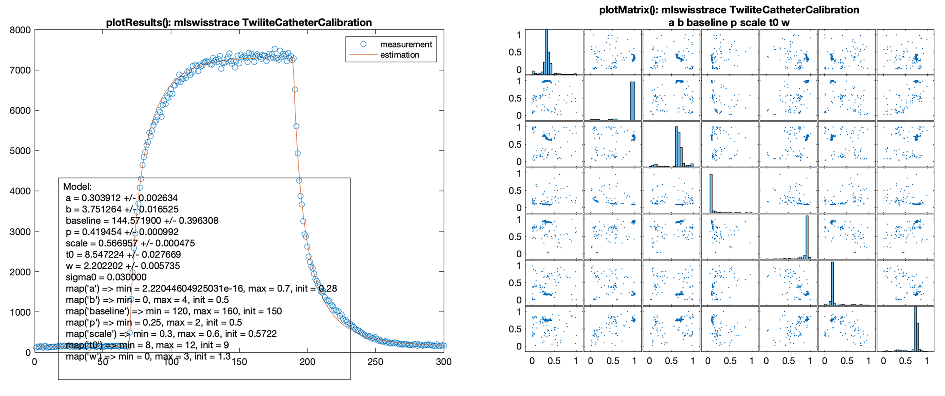
\includegraphics[angle=0,width=17cm]{TwiliteCatheterCalibration}
\caption{Left panel shows emissions, model fit and best parameters.  Right panel
shows the covariance of distributions.  Similar results were obtained for each of the 
trials of impulse-response.}
\label{fig:twiliteCC_LRw}
\end{figure*}

%%%%%%%%%%%%%%%%%%%%%%%%%%%%%%%%%%%%%%%%%%%%%%%%%%%%%%%%%%%%%%%%%%%%%%%%%%%%%
%\section{The Bibliography}
%Bibliographic entries may be made either in the `.tex' file itself or within a
%separate `.bib' file which gets attached during process of building a
%final PDF document.  This latter method is the preferred method and is
%then one used in this template by default.  An example of the
%alternative style, currently commented out,  is contained in the `.tex' source file.

%%%%%%%%%%%%%%%%%%%%%%%%%%%%%%%%%%%%%%%%%%%%%%%%%%%%%%%%%%%%%%%%%%%%%%%%%%%%%
% Place all of the references you used to write this paper in a file
% with the same name as following the \bibliography command
%%%%%%%%%%%%%%%%%%%%%%%%%%%%%%%%%%%%%%%%%%%%%%%%%%%%%%%%%%%%%%%%%%%%%%%%%%%%%

%\bibliography{sample}

%\bibliographystyle{prsty}
%\begin{thebibliography}{99}
%\bibitem{melissinos1966}Melissinos, A.C., Experiments in Modern
%  Physics - 1st Edition, Academic Press,  [1966]
%\bibitem{melissinos2003}Melissinos, A.C., Napolitano, J.,  Experiments in Modern
%  Physics - 2nd Edition, Academic Press,  [2003]
%\bibitem{bevington2003}Bevington and Robinson, Data Reduction and
%  Error Analysis for the Physical Sciences - 3rd Edition, McGraw-Hill,
%  [2003]
%\bibitem{pritchard1990}Professor D. Pritchard, Personal Communication
%\end{thebibliography}

%%%%%%%%%%%%%%%%%%%%%%%%%%%%%%%%%%%%%%%%%%%%%%%%%%%%%%%%%%%%%%%%%%%%%%%%%%%%%
\clearpage
\appendix





% Surround figure environment with turnpage environment for landscape
% figure
% \begin{turnpage}
% \begin{figure}
% \includegraphics{}%
% \caption{\label{}}
% \end{figure}
% \end{turnpage}

% tables should appear as floats within the text
%
% Here is an example of the general form of a table:
% Fill in the caption in the braces of the \caption{} command. Put the label
% that you will use with \ref{} command in the braces of the \label{} command.
% Insert the column specifiers (l, r, c, d, etc.) in the empty braces of the
% \begin{tabular}{} command.
% The ruledtabular enviroment adds doubled rules to table and sets a
% reasonable default table settings.
% Use the table* environment to get a full-width table in two-column
% Add \usepackage{longtable} and the longtable (or longtable*}
% environment for nicely formatted long tables. Or use the the [H]
% placement option to break a long table (with less control than
% in longtable).
% \begin{table}%[H] add [H] placement to break table across pages
% \caption{\label{}}
% \begin{ruledtabular}
% \begin{tabular}{}
% Lines of table here ending with \\
% \end{tabular}
% \end{ruledtabular}
% \end{table}

% Surround table environment with turnpage environment for landscape
% table
% \begin{turnpage}
% \begin{table}
% \caption{\label{}}
% \begin{ruledtabular}
% \begin{tabular}{}
% \end{tabular}
% \end{ruledtabular}
% \end{table}
% \end{turnpage}


\end{document}
